\section{Leading order, two flavor pion stars}


\subsection{Equation of state}
The free energy density of two-flavor chiral perturbation theory, to leading-order and at $T = 0$, is
%
\begin{equation}
    \Eff = - f^2 \left(\bar m^2 \cos \alpha + \frac{1}{2} \mu_I^2 \sin^2 \alpha\right).
\end{equation}
%
The $\alpha$ parameter is determined by minimizing $\Eff$ for a given value of $\mu_I$,
%
\begin{equation}
    \pdv{\Eff}{\alpha} = f^2 \left(\bar m^2 - \mu_I^2 \cos \alpha\right) \sin(\alpha) = 0.
\end{equation}
%
This gives an explicit formula for $\alpha$ in terms of $\mu_I$.
We are only interested in the phase where $\mu_I \geq \bar m$, where this solution is
%
\begin{align}
    \label{alpha as function of mu lowest order}
    \cos \alpha = \frac{\bar m^2}{\mu_I^2}.
\end{align}
%
We introduce a dimensionless variable $x^2 = \cos(\alpha) = \bar m^2 / \mu_I^2$.
This variable has the domain $[0, 1]$.
By an argument using a right triangle, we can verify that $\cos \alpha = x^2$ implies that $\sin^2 \alpha = 1 - x^4$.
Substituting the dimensionless variable into the free energy density, we get 
%
\begin{equation}
    \Eff = - \frac{u_0}{2} \left( x^2 + \frac{1}{x^2} \right).
\end{equation}
%
We have introduced the characteristic energy density $u_0 = \bar m^2 f^2$.
As we found in \autoref{section: cold fermi star}, the pressure is given by negative the free energy density, normalized to $\mu_I = \bar m$, or $x = 1$.
We choose $p_0 = u_0$, so the dimensionless pressure can be written
%
\begin{equation}
    \label{pressure leading order chpt}
    \tilde p = -\frac{1}{p_0} \left(\Eff - \Eff_{x=1}\right) 
    = \frac{1}{2} \left( x^2 + \frac{1}{x^2} - 2 \right).
\end{equation}
%
The charge density corresponding to a chemical potential is given by minus the derivative of the free energy with respect to that chemical potential. 
We must, however, not assume any dependence of $\alpha$ on $\mu_I$ when taking this derivative.
The isospin density therefore is
%
\begin{equation}
    n_I = -\pdv{\Eff}{\mu_I} = ^2 \mu_I^2 \sin^2 \alpha 
    = 
    \frac{u_0}{\mu_I} \left(\frac{1}{x^2} - x^2\right).
\end{equation}
%
With this, the dimensionless energy density at $T = 0$ is
%
\begin{equation}
    \label{energy density leading order chpt}
    \tilde u = - \tilde p + \frac{\mu_I n_I}{u_0}
    = \frac{1}{2} \left( 2 + \frac{1}{x^2} - 3 x^2\right).
\end{equation}
% 
The ratio of pressure to energy density is
%
\begin{equation} 
    \label{pressure energy ratio leading order chpt}
    \frac{p}{u} = \frac{1- 2x^2 + x^4  }{1 + 2x^2 -3x^4 }.
\end{equation}
%
In the ultrarelativistic limit, where $\mu_I \rightarrow \infty$ and thus $x \rightarrow 0$, we get $p / u = 1$, or $p = u$.
In the non-relativisitc limit, that is $x^{-2} = 1 + \epsilon$, $\epsilon \ll 1$, we get $\tilde p = \epsilon^2 / 2 $, and $\tilde u = 2\epsilon$.
Thus, the equation of state has the NR-limit $\tilde u = 2 \sqrt 2 \sqrt{\tilde p}$.
\autoref{fig: equation of state pions} shows the equation of state in two different regimes, and compares it with the ultrarelativistic and non-relativistic limit.
\todo[inline]{Er UR-grensen gyldig, eller feiler chpt?}
\todo[inline]{Sammenilign med polytrope}



\begin{figure}[h]
    \centering
    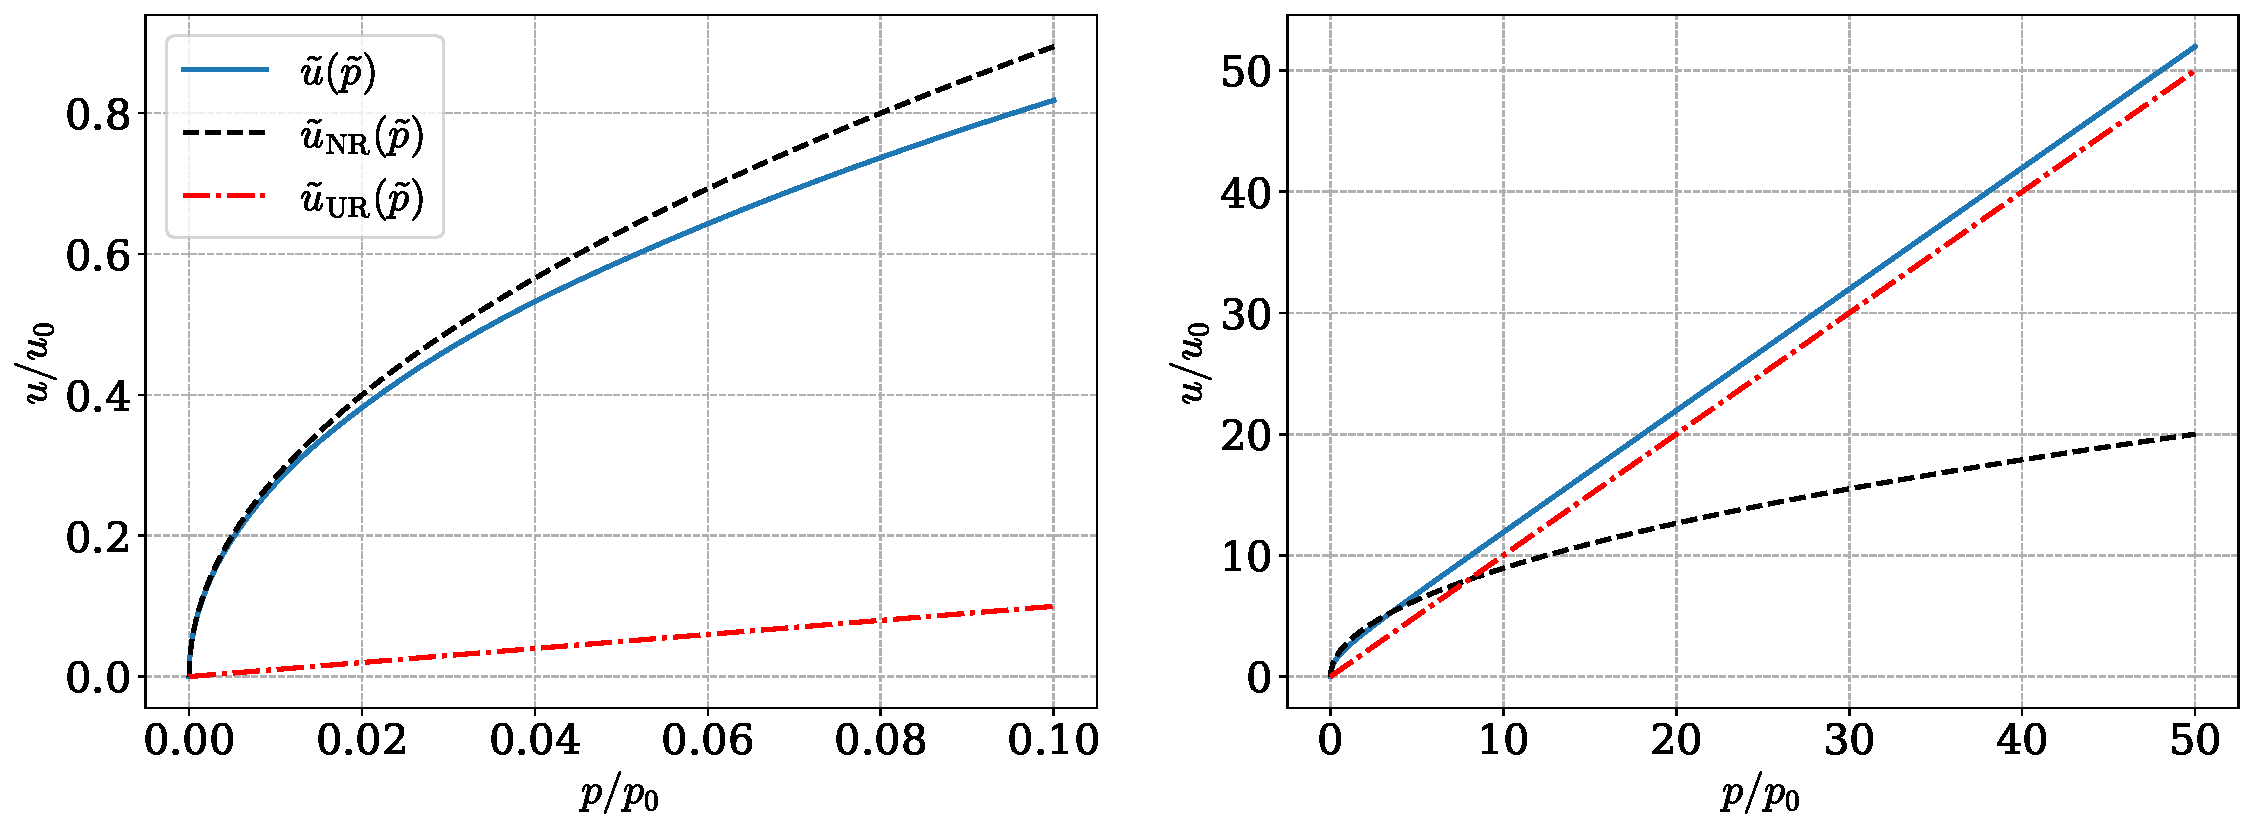
\includegraphics[width=0.95\textwidth]{../scripts/figurer/pion_star/pion_eos.pdf}
    \caption{
        This plot shows the leading order equation of state of two-flavor chiral perturbation theory and compares it with the ultrarelativistic and non-relativistic limit, shown as dashed lines. The $x$-axis shows the pressure normalized to $p_0$, while the $y$-axis shows the energy density normalized to $u_0$.
    }
    \label{fig: equation of state pions}
\end{figure}


\subsection{Units}

The characteristic mass and length, as discussed in \autoref{section: TOV equation}, are found by setting $k_1 = k_2 = k_3 = 1$.
These are the dimensionless constants of the TOV equation, \autoref{dimensionless constants TOV}.
At tree-level, the bare constants $f$ and $\bar m$ are related to physical constants by $f = f_\pi$ and $m = m_\pi$, the pion decay constant and the pion mass.
Using the values for $f_\pi$ and $m_\pi$ as given in \autoref{section: units} and reinstating $c$ and $\hbar$, these quantities are give in SI-units by
%
\begin{align}
    u_0 & =m_\pi^2 f_\pi^2 \frac{c}{\hbar^3}
    = 3.216\cdot 10^{33} \, \text{J}\,\text{m}^{-3}, \\
    m_0 & = \frac{c^4}{\sqrt{\frac{4 \pi}{ 3} u_0 G}} = 64.21\, M_\odot, \\
    r_0 & = \frac{G}{c^2} m_0 = 94.79 \, \text{km}.
\end{align}
%
We, therefore, expect both the radius and mass of the pion star to be around one order of magnitude larger than the star made up of cold neutrons.

\subsection{Results}

The code used for obtaining numerical results is discussed in \autoref{appendix: code}.

\autoref{fig: pressure and mass for pion star} show the pressure and mass as a function of radius for a range of central pressures.
The quantities are normalized to the stellar radius, stellar mass, and central pressure, respectively.
The black dashed line corresponds to the configuration with the maximum mass.
We see that both the pressure and mass distribution are very similar for stars with a mass less than the maximum.
As the central pressure increase beyond that of the star with maximum mass, the pressure gradient close to the center grows sharply.
This is similar to what we saw in the case of an incompressible fluid, \autoref{subsection: incompressible fluid}.

\begin{figure}[!h]
    \centering
    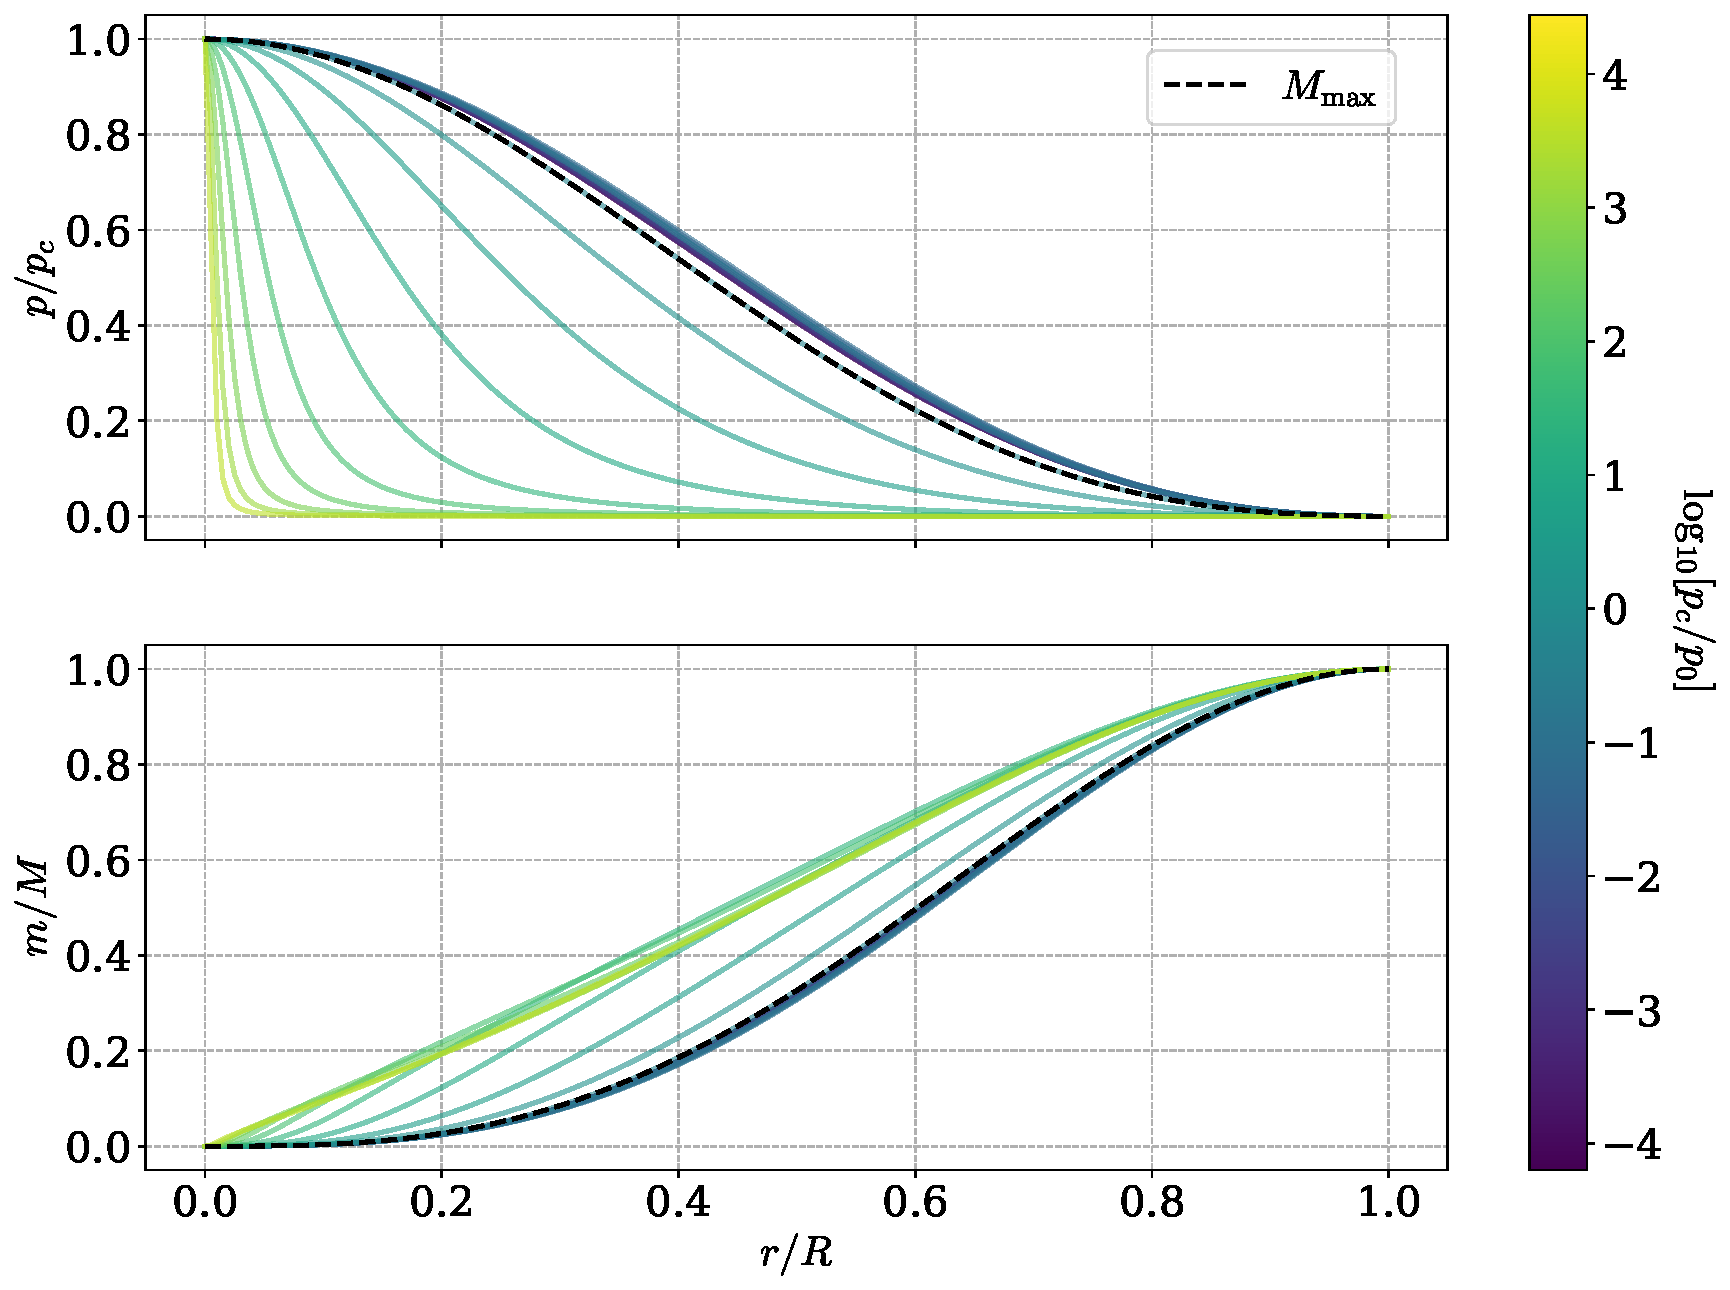
\includegraphics[width=0.8\textwidth]{../scripts/figurer/pion_star/pressure_mass_pion_star.pdf}
    \caption{
        Top: The pressure normalized to the central pressure, as a function of radius, normalized to the stellar radius.
    Bottom: The mass, normalized to stellar mass, within a radius $r$, normalized to the stellar radius.
    Both plots show a range of stars with different central pressures, indicated by the color.
    The black dashed line corresponds to the star with the largest mass.
    }
    \label{fig: pressure and mass for pion star}
\end{figure}

\begin{figure}[!h]
    \centering
    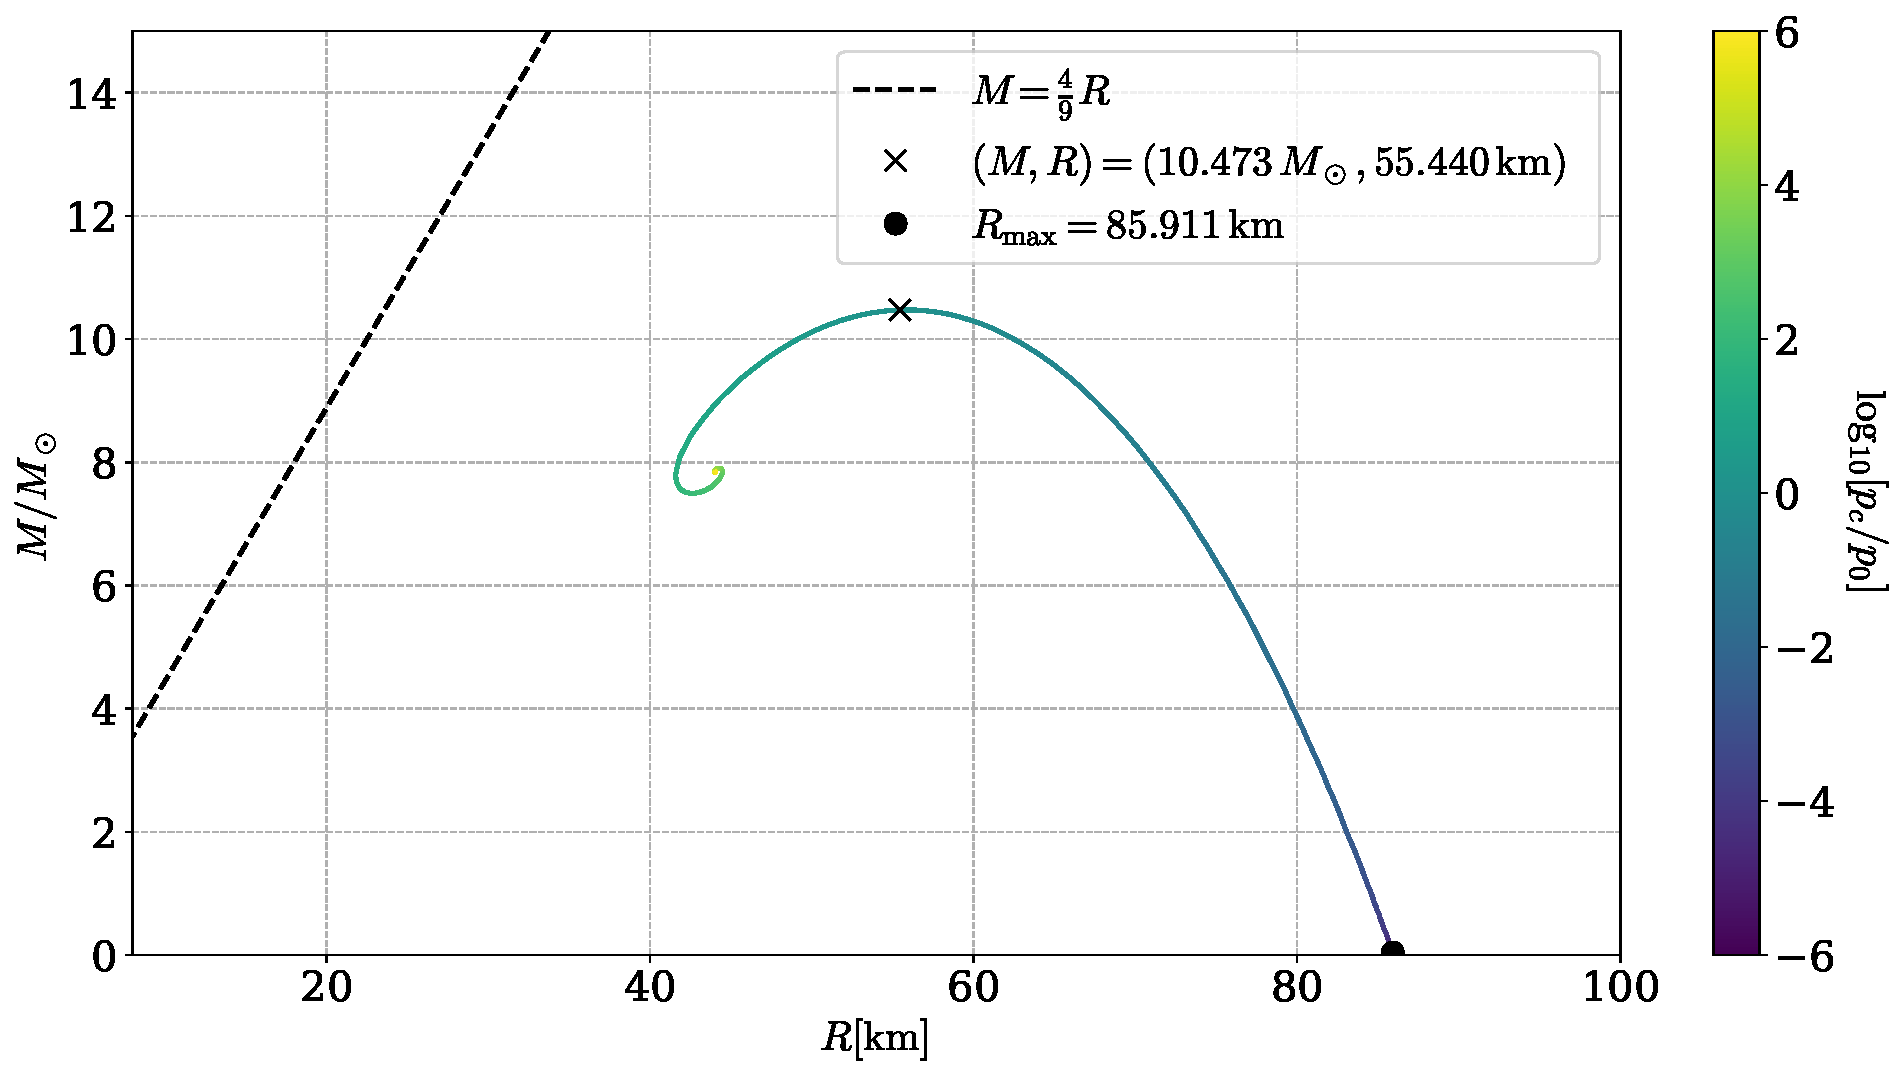
\includegraphics[width=0.85\textwidth]{../scripts/figurer/pion_star/mass_radius_pion_star.pdf}
    \caption{
        The plot shows the relationship between the mass and radius of a pion star. Mass is given in units of solar masses, while the radius is measured in kilometers.
        This line is parameterized by the central pressure $p_c$ of the star, as indicated by the color gradient.
        The dashed black line indicates the theoretical maximum mass for a given radius, and the configuration above it will collapse to a black hole.
        }
        \label{fig: mass-radius relation pion star}
\end{figure}

\begin{figure}[!h]
    \centering
    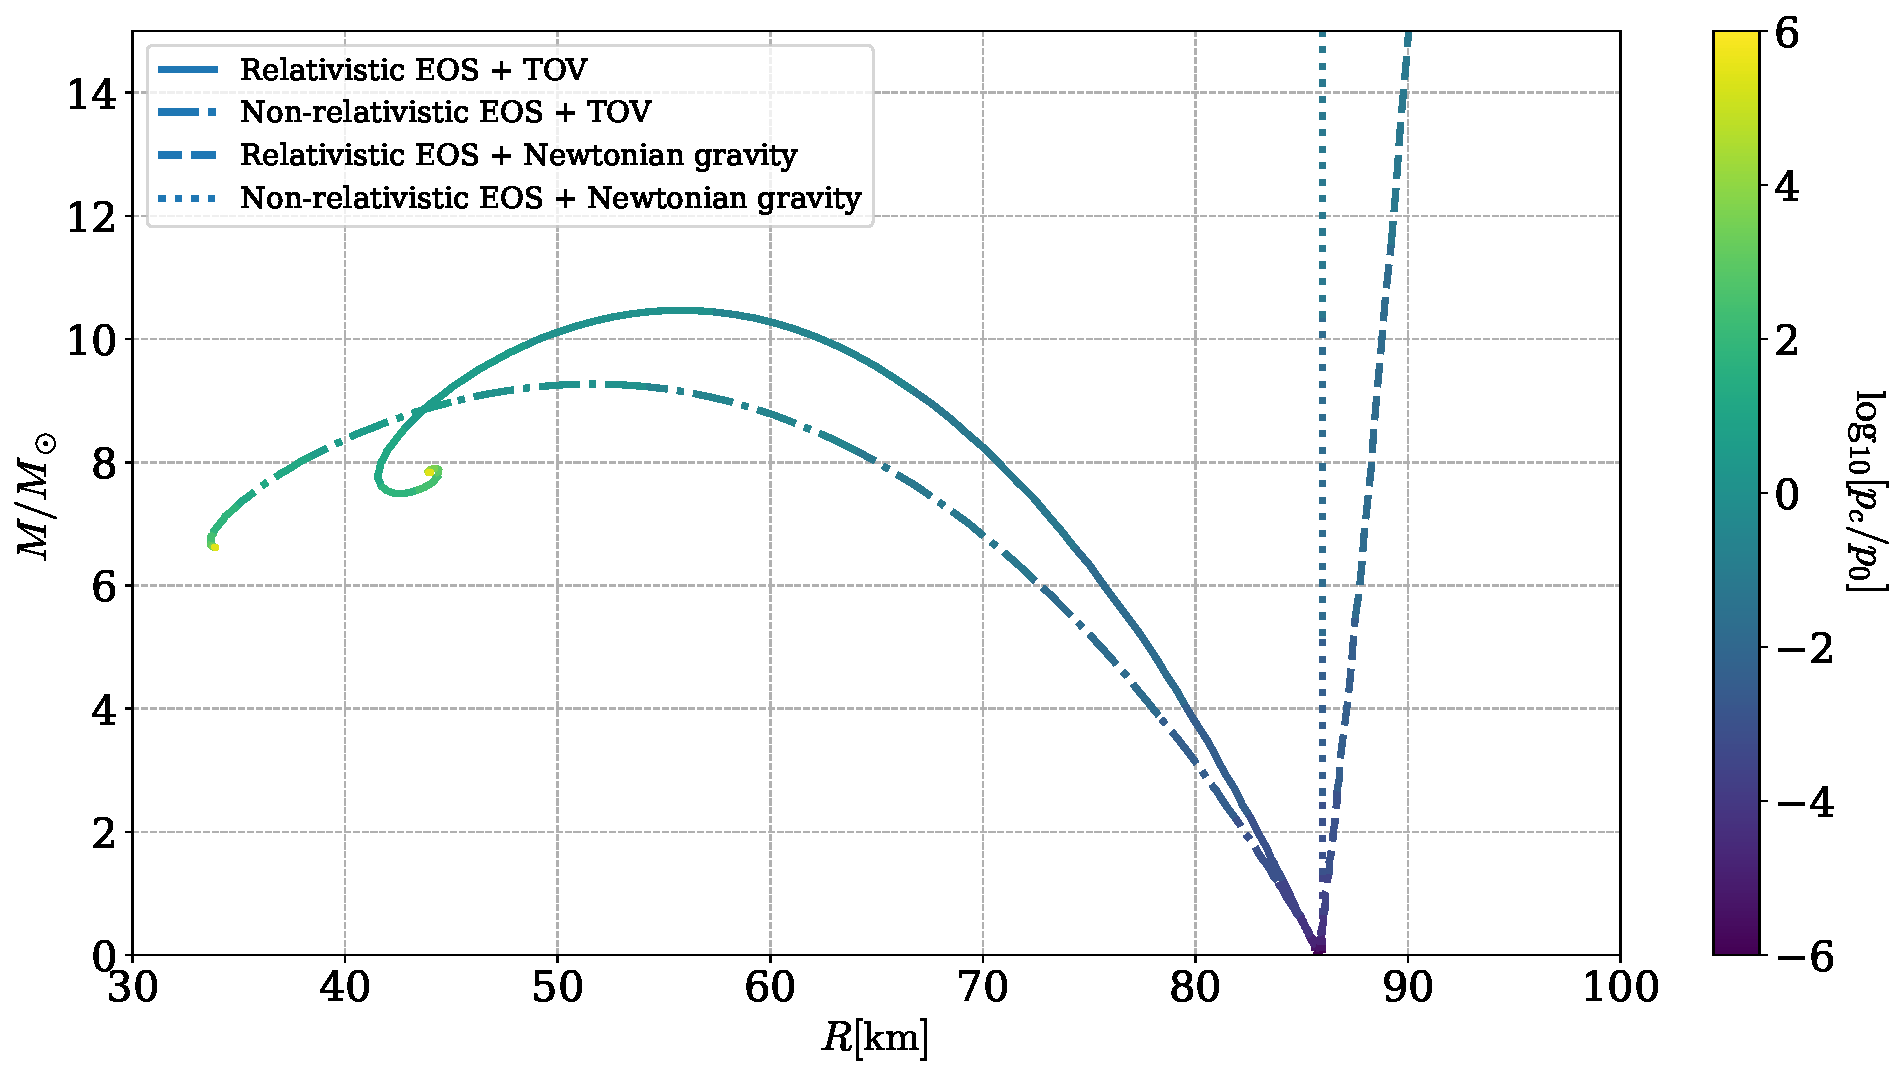
\includegraphics[width=0.85\textwidth]{../scripts/figurer/pion_star/mass_radius_comparison.pdf}
    \caption{
        The plot compares the mass-radius relationship of the pion star from the full equation of state and the TOV-equation with various limits.
        }
        \label{fig: mass-radius relation pion star comparison}
\end{figure}


\autoref{fig: mass-radius relation pion star} shows the mass-radius relationship for the pion star using the leading order free energy density of two-flavor chiral perturbation theory.
As in the case of the neutron star, it has a maximum mass, in this case of $M_\text{max} 10.47\, M_\odot$.
What distinguishes this from the case of the neutron star, however, is the fact that in the limit of low central pressure, the distribution apparently approaches a maximum radius of $R = 85.95 \, \text{km}$.
\todo{Hvorofor? Fordi eos er så lite stiv?}
\autoref{fig: mass-radius relation pion star comparison} compares the mass-radius relation from the full equation of state and TOV equation with various limits.
We see that  when using the Newtonian limit of the TOV equation, \autoref{Newtonian limit TOV}, the radius is either constant or increasing as the mass increases, in contrast to the result when using the TOV equation, as well as the neutron star.
\todo[inline]{sammenlign med polytrope}
\todo[inline]{Vis kjemisk potensial}



\FloatBarrier
\subsection{Including electromagnetic contributions}

From \autoref{static lagrangian with EM}, the free energy density, including electromagnetic interactions, is
%
\begin{equation}
    \Eff =
    - f^2 \left[
        \bar m^2 \cos \alpha 
        + \frac{1}{2} \mu_I^2 \sin^2 \alpha
        + \frac{1}{2} \Delta m_\pm^2 \left(\cos^2 \alpha - \frac{4}{9}\right)
    \right],
\end{equation}
%
Free energy minimization now gives
%
\begin{equation}
    \frac{1}{u_0}\pdv{\Eff}{\alpha}
    = 
    \left[ \left( \frac{1}{x^2} - \Delta \right) \cos \alpha - 1\right] \sin \alpha = 0.
\end{equation}
%
Here, $x$ is defined as before, and we introduced the new quantity $\Delta = \Delta m_{\pm}^2 / \bar m^2= 0.06916 $.
We see that $\alpha = 0$ is the only solution for $x^{-2} = \mu_I^2 / \bar m^2 < 1 + \Delta$.
The phase transition is raised to $\mu_I = \bar m \sqrt{1 + \Delta}$, the charged pion mass.
This gives the new solution
%
\begin{equation}
    \cos \alpha = \frac{x^2}{1 - \Delta x^2}.
\end{equation}
%
\todo[inline, color=red]{Fiks faktor to forran delta, kjør kode på nytt}
This reduces to our old solution for $\Delta = 0$, as it should.
With the same procedure as in the last section, we get the pressure and energy density
%
\begin{align}
    \tilde p_\text{EM} \
    & = \frac{1}{2} 
    \left[
        \frac{1}{x^2} 
        + \frac{x^2}{1 - 2x^2 \Delta} 
        - 2(1 + \Delta)
    \right], \\
    \tilde u_\text{EM}
    &= \frac{1}{2} 
    \left[
        \frac{1}{x^2} 
        - x^2 \frac{3 - 2 \Delta x^2}{(1 - 2 \Delta x^2)^2}
        + 2(1 + \Delta)
    \right].
\end{align}
%

\begin{figure}[!htb]
    \centering
    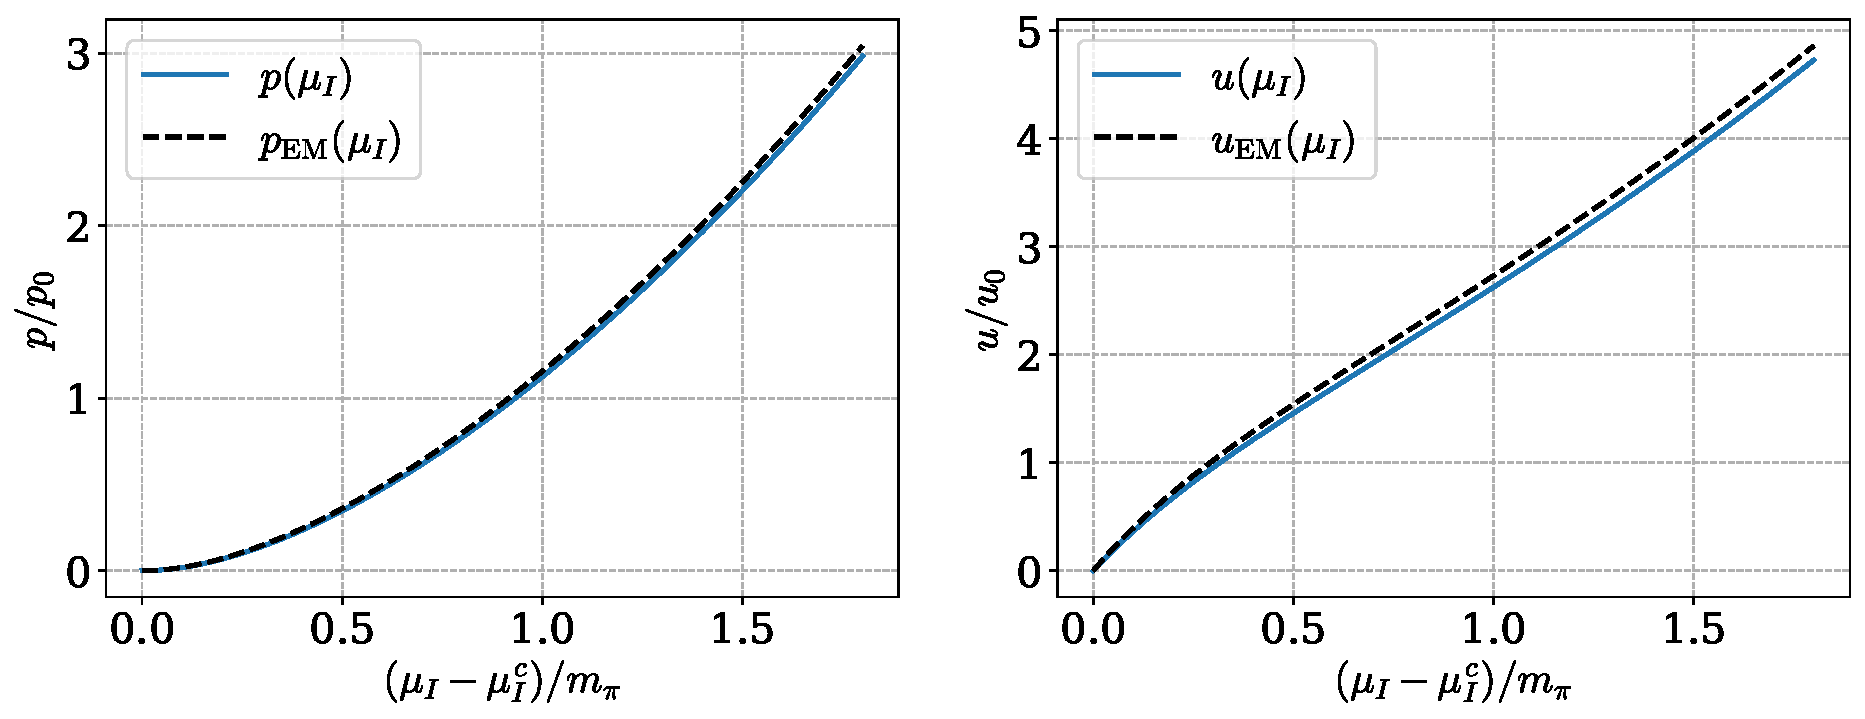
\includegraphics[width=0.95\textwidth]{../scripts/figurer/pion_star/pion_up.pdf}
    \caption{text
        }
        \label{fig: pressure and energy with EM interaction}
\end{figure}



\begin{figure}[!htb]
    \centering
    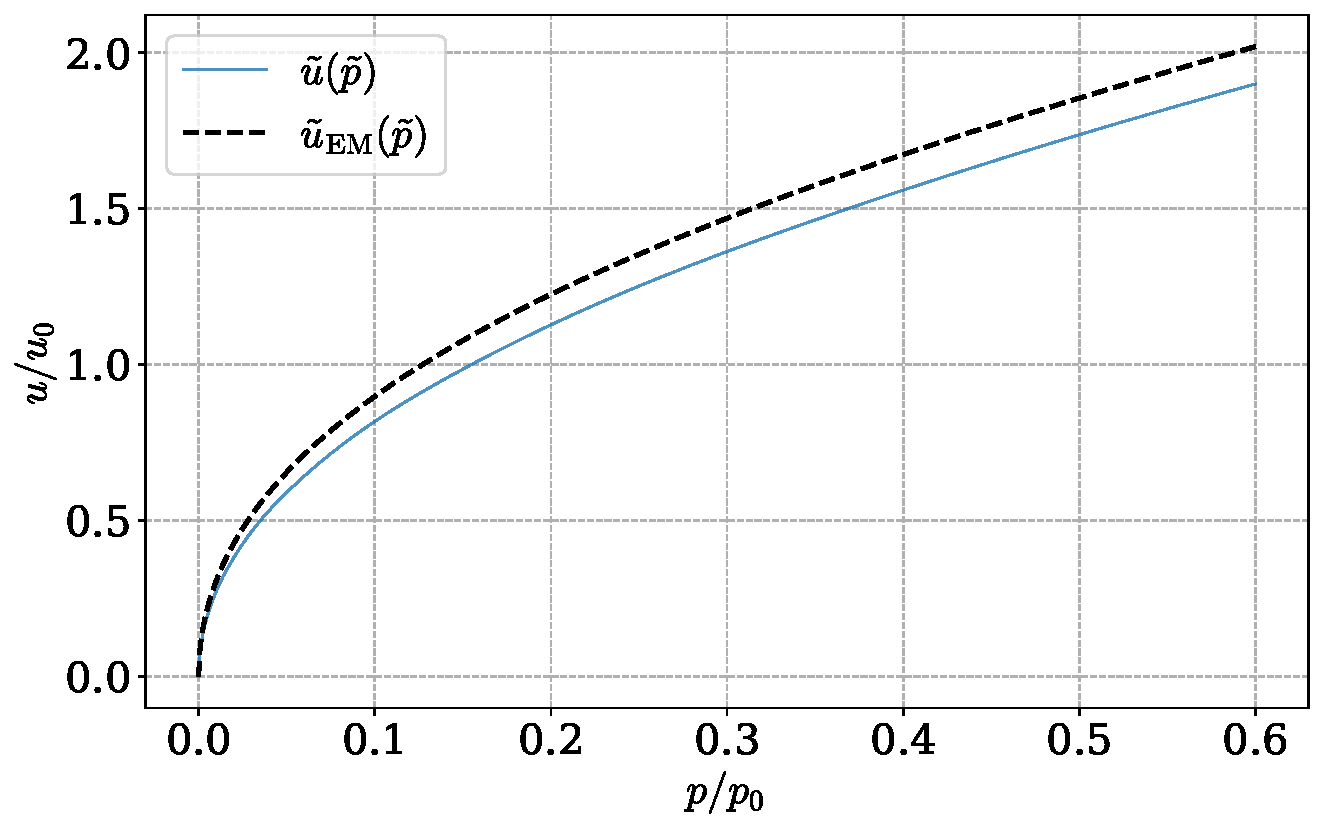
\includegraphics[width=0.65\textwidth]{../scripts/figurer/pion_star/pion_eos_EM.pdf}
    \caption{c}
    \label{fig: eos chpt em interaction}
\end{figure}

In the limit $\Delta = 0$, these reduce to \autoref{pressure leading order chpt} and \autoref{energy density leading order chpt}.
The ultra-relativisitc limit, that is for  $x \ll 1$, the behavior is the same as before, and we therefore again approach $p = u$.
\autoref{fig: pressure and energy with EM interaction} shows the pressure and energy density, normalized to their characteristic quantities, as a function of chemical potential above the critical value, normalized to $\bar m$.
The critical value of the chemical potential, $\mu_I^c$, is the point where we get a new solution $\alpha\neq 0$.
Normalized to $\bar m$, this is $1$ when electromagnetic interactions are ignored, and $\sqrt{1 + 2 \Delta}$ when they are accounted for.



\autoref{fig: mass-radius relation leading order pion star with em interaction} shows the mass-radius reaction of the pion star when the electromagnetic interaction is taken into account.
We see that the shape of the curve has not changed much from our earlier result. 
Both the maximum mass and radius are slightly smaller.
The result with and without electromagnetic interaction is compared in \autoref{fig: mass-radius relation comparison}.


\begin{figure}[!htb]
    \centering
    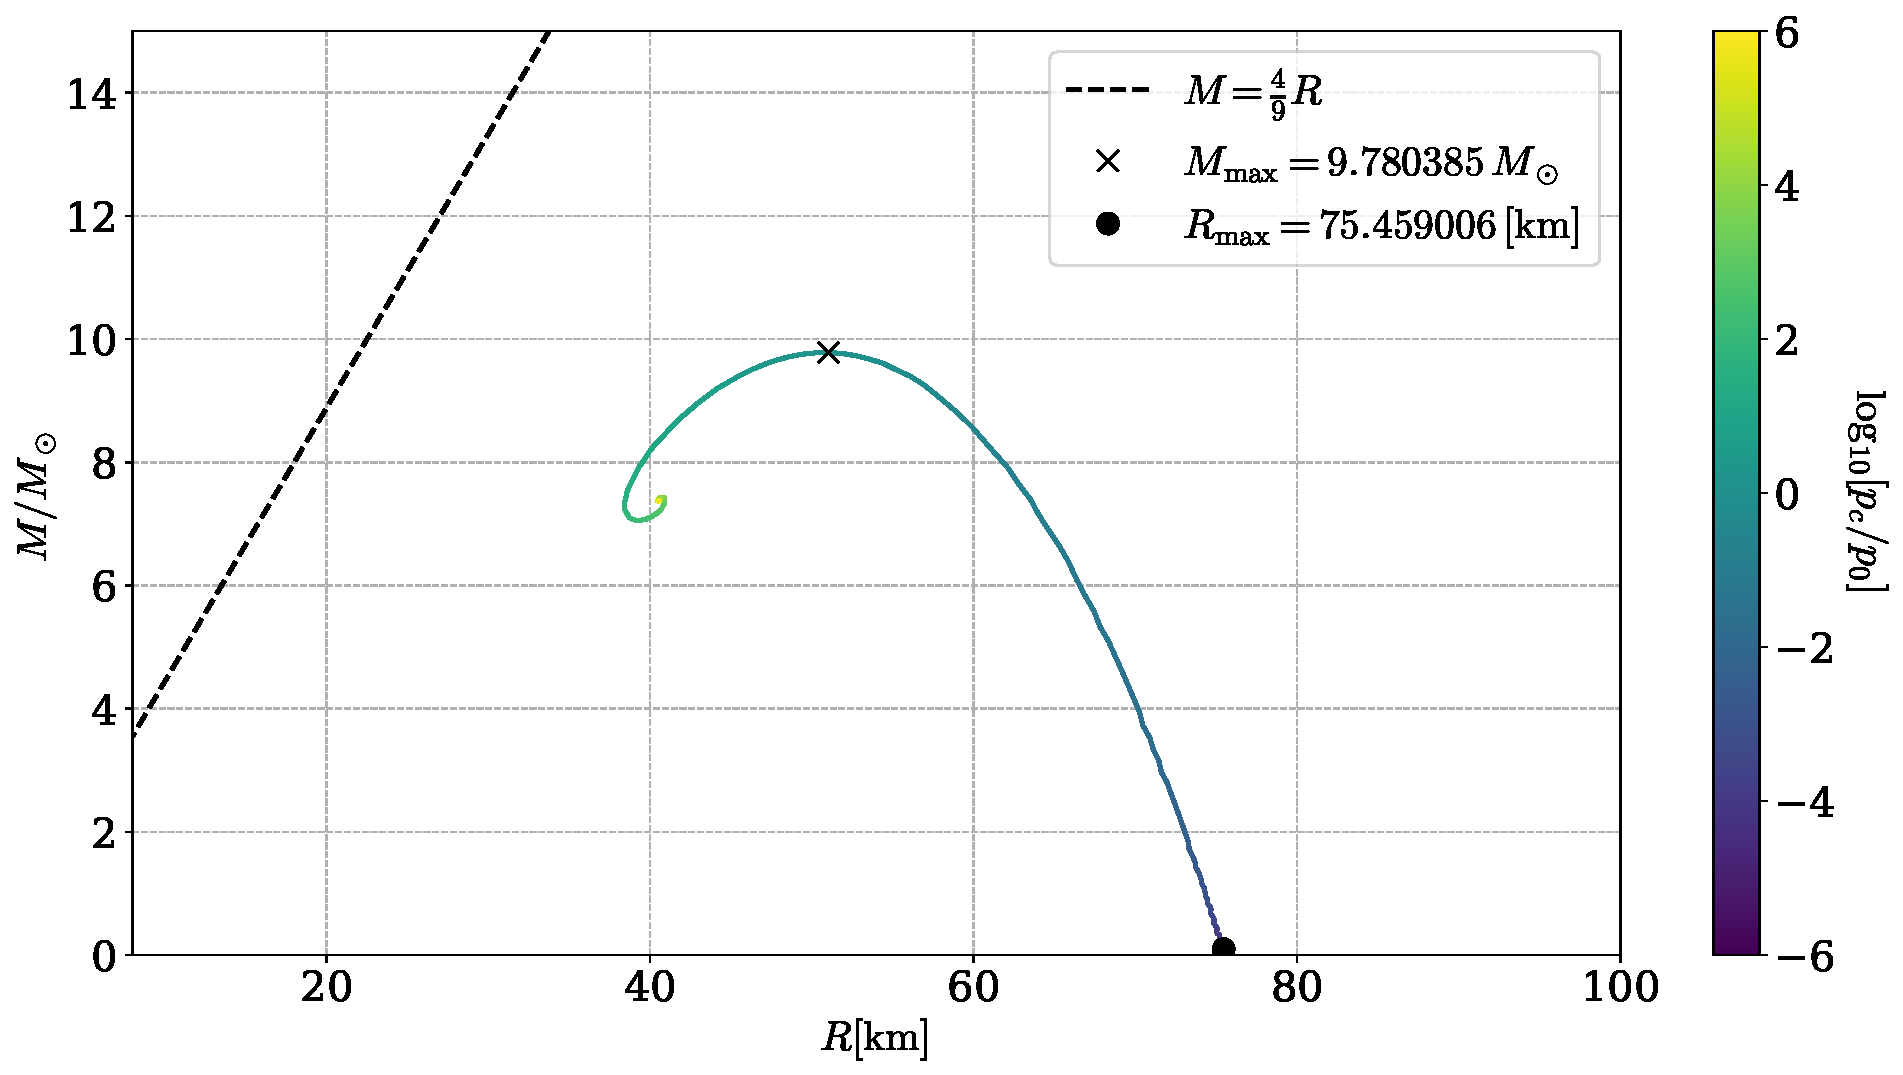
\includegraphics[width=0.85\textwidth]{../scripts/figurer/pion_star/mass_radius_pion_star_EM.pdf}
    \caption{a }
    \label{fig: mass-radius relation leading order pion star with em interaction}
\end{figure}


\begin{figure}[!htb]
    \centering
    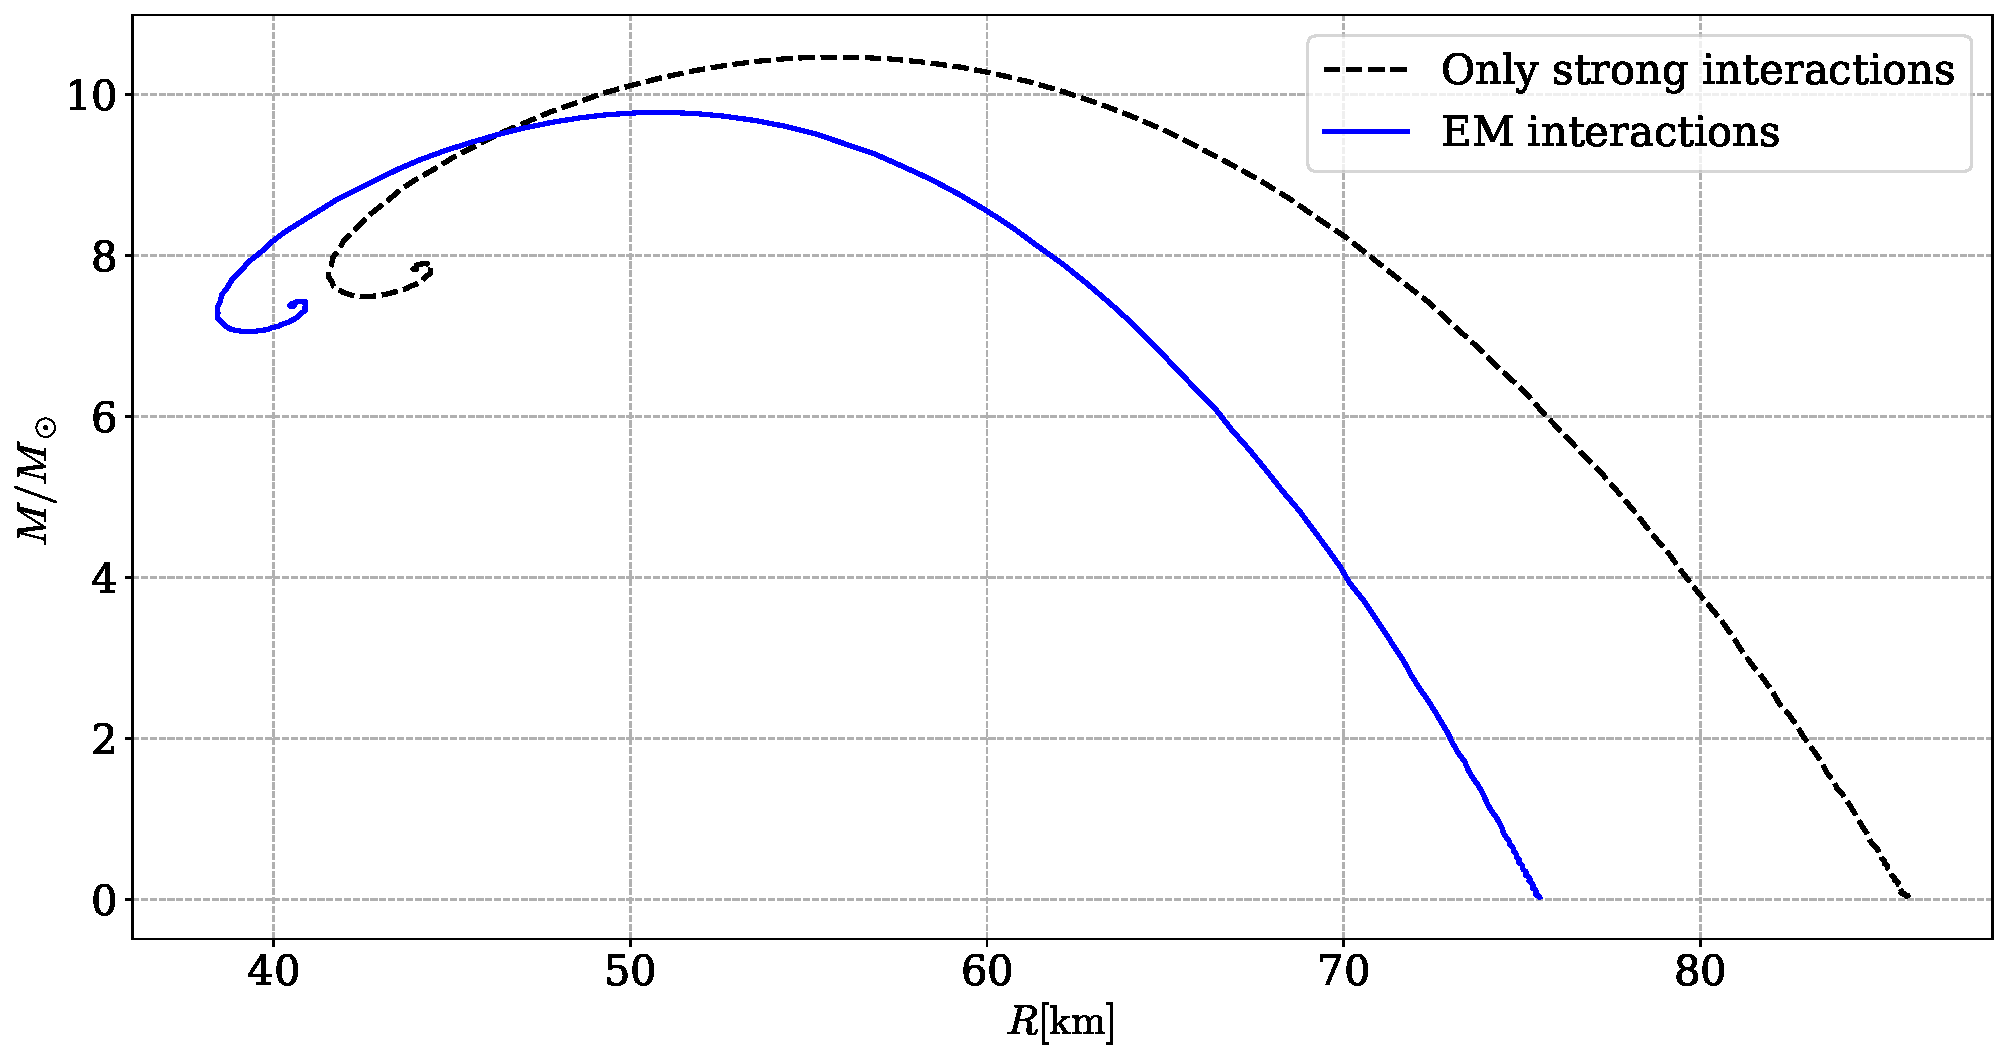
\includegraphics[width=0.85\textwidth]{../scripts/figurer/pion_star/mass_radius_pion_star_compare.pdf}
    \caption{b
        }
        \label{fig: mass-radius relation comparison}
\end{figure}
